\documentclass[tikz,border=3mm,convert={density=960,outfile=\jobname.png}]{standalone}
%\documentclass[tikz,border=3mm]{standalone}
\usetikzlibrary{shadings,fadings,calc}
\begin{document}
	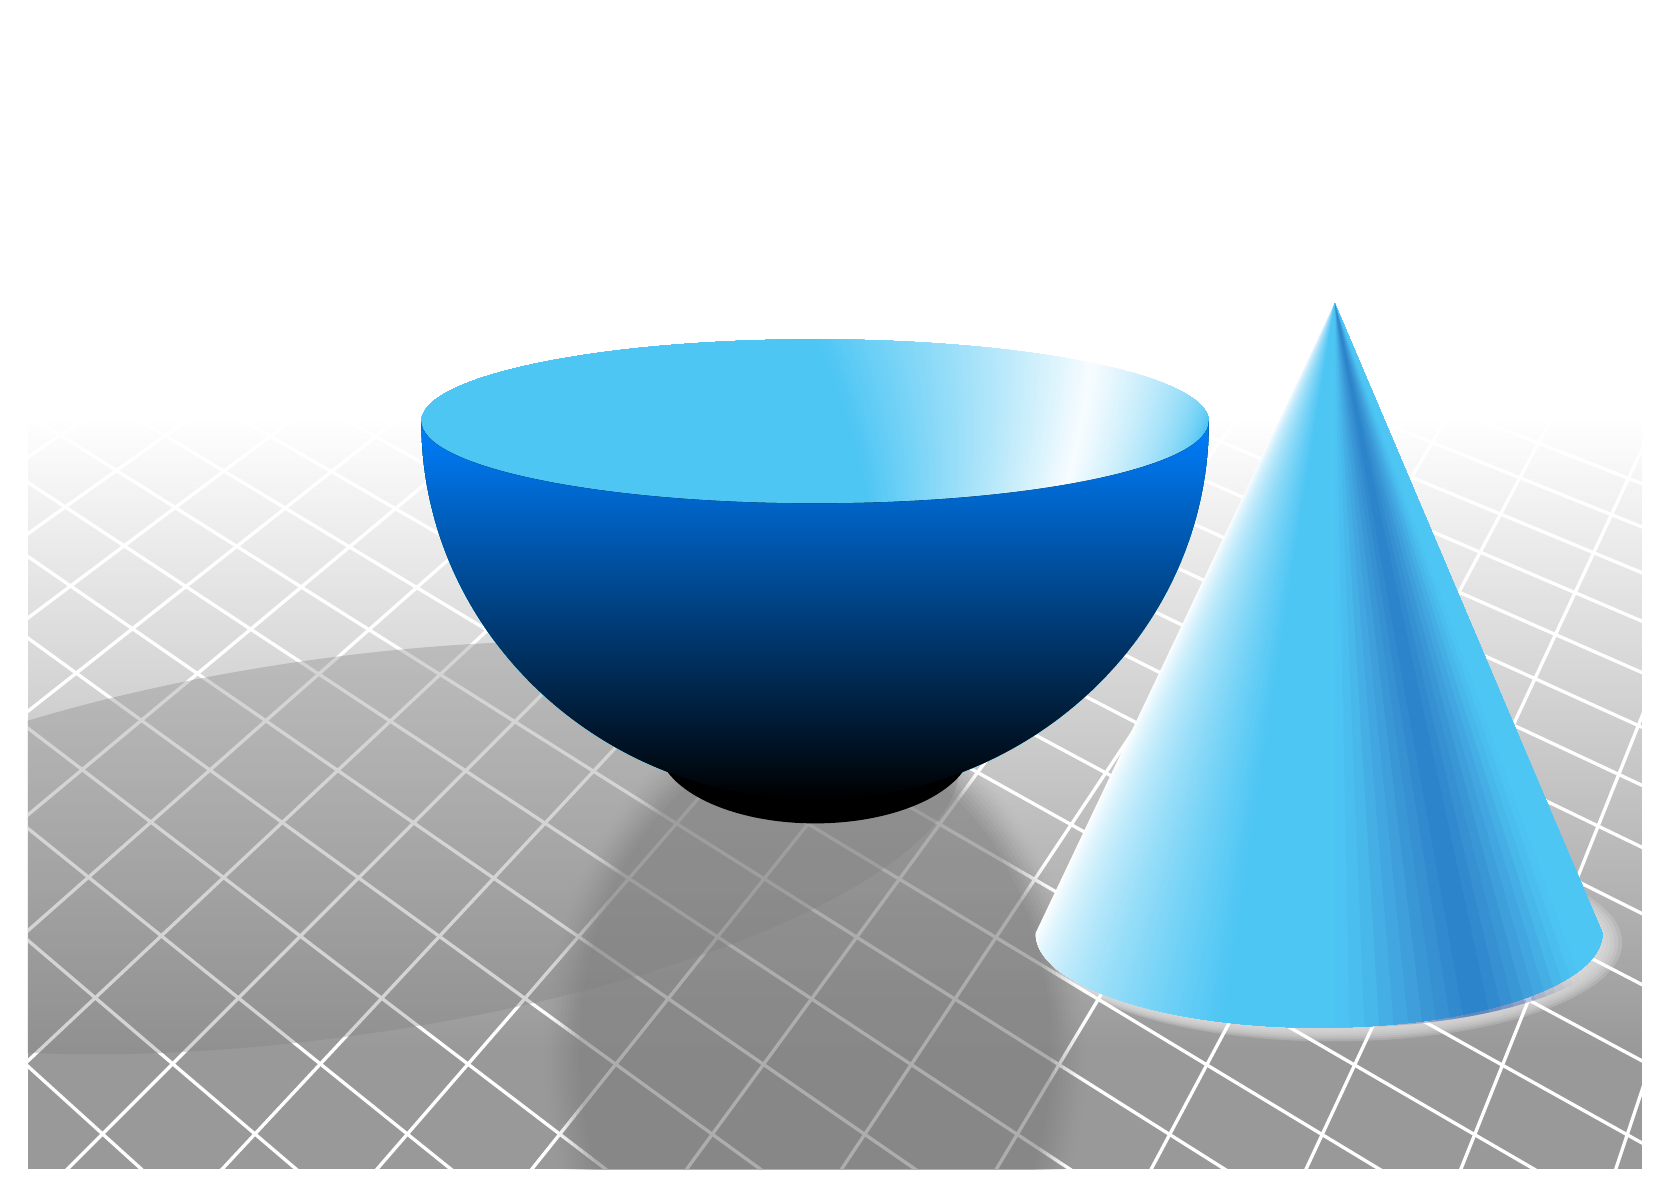
\begin{tikzpicture}[>=stealth,line join=round,line cap=round,font=\footnotesize,scale=1]
		\clip (0,0.5)rectangle(20.5,15);
		\fill[gray!80] (0,0.5)rectangle(20.5,15);
		\foreach \i in {0,2,4,...,44}{
			\draw[very thick,white] (\i,0)--(-30,29) (\i-20,0)--(30,30);
		}
		\fill[white] (0,15)rectangle(20.5,10);
		\fill[white,path fading=south] (0,10)rectangle(20.5,2);
		\foreach \x in {1,...,10}{
			\pgfmathsetmacro\n{11-\x}
			\fill[white,opacity=\x/60] (12.9,3.38)arc(-180:180:{3.7-\n/40} and {1.28-\n/40});
		}
		\foreach \n in {1,...,10}{
			\fill[gray,opacity=\n/60] (10,2)ellipse({3.5-\n/20} and {4.5-\n/20});
		}
		\fill[gray,opacity=1/3,rotate=8,yscale=.8] (12.5,5)arc(0:360:8 and 3);
		\foreach \x in {100,99,...,30}{
			\fill[white!\x!cyan] (15,10)arc(0:-90:5 and 4.8)to[bend right=25]($(10,10)+({\x/1.5-19}:5 and 5/4.8)$)arc({\x/1.5-19}:0:5 and 5/4.8)--cycle;
			\fill[white!\x!cyan] ($(10,10)+({286/3-\x/1.5+14.5}:5 and 5/4.8)$)to[bend left=25](10,5.2)arc(-90:-180:5 and 4.8)arc(-180:-270:5 and 5/4.8)arc(90:{286/3-\x/1.5+14.5}:5 and 5/4.8)--cycle;
			\fill[white!\x!cyan] (16.6,11.5)--(20,3.5)arc(0:{-\x-80}:3.6 and 1.2)--cycle;
		}
		\fill (10,5.9)ellipse(2 and 1.8/1.79);
		\fill[bottom color=black,top color=blue!50!cyan] (15,10)arc(0:-180:5 and 4.8)arc(-180:0:5 and 5/4.8)--cycle;
		\foreach \x in {1,...,10}{
			\pgfmathsetmacro\y{\x*5}
			\pgfmathsetmacro\n{11-\x}
			\fill[cyan!\y!blue,opacity=\x/60] (16.6,11.5)--($(16.6,3.5)+({-60+3*\n}:3.6 and 1.2)$)arc({-60+3*\n}:{-60-3*\n}:3.6 and 1.2)--cycle;
		}
	\end{tikzpicture}
\end{document}